\documentclass[12pt]{article}
\usepackage[onehalfspacing]{setspace}
\usepackage{dcolumn}
\usepackage[left=1in, top=1in, bottom=1in]{geometry}
\usepackage{graphicx}
\usepackage[table,xcdraw]{xcolor}
\usepackage{longtable}
\usepackage{float}
\usepackage{listings}
\usepackage{xcolor}
\usepackage{amsmath}
\usepackage{amsfonts}
\usepackage{amssymb}


\begin{document}

\title{Predictive Analytics - Individual Assignment}
\maketitle
{\setlength{\parindent}{0cm}
\section*{Executive Summary}
Looking at monthly temperature data from Melbourne airport, we are able to analyse trends that suggest global warming and climate change. Weather data is highly seasonal however, using time series decompositions we are able to separate the seasonality and observe a mostly positive trend in both the mean maximum and temperature difference since 1970. The use of regression analysis helps us to estimate this effect to be a yearly linear increase of approximately $0.024^\circ C$ per year in the mean maximum temperature and $0.042^\circ C$ in the temperature difference. Moreover, the use of forecasts allows us to observe that these trends are likely to continue into the future. The following report goes through the process of decomposition, regression and forecasting in more detail while also elucidating the choices in our approach.

\section*{Discussion}
Global warming is the increase of the general temperature over time. Obviously temperature undergoes seasonal temperature changes each year, but global warming states that despite this seasonality, there is an overall increasing trend. The monthly temperature data captured at Melbourne Airport can give us an idea of this effect since 1970. As the main cause of global warming is considered to be our rapid increase in $CO_2$ emissions since the industrial revolution, we can't compare the current trend to any weather trends before the industrial revolution without data from that period. However, it has been largely established that with the exception of a few ice ages, the temperature has stayed generally stable so finding an upwards trend in our data should suggest some sort of global warming.\\

Recent discussion has shifted away the focus from global warming over to climate change, which is inclusive of global warming. Essentially, climate change is any indication that the weather is becoming more variable, i.e. more frequent extreme weather events, colder Winters and warmer Summers. Thus, identifying trends in the difference between the highest and lowest temperatures each month can be seen as evidence of climate change.\\

Looking at the overall plot of the temperature features since 1970 (see appendix figure 1), the seasonality is obvious in each feature however, this makes any trend hard to see with the naked eye, especially since for global warming to be evident, we only need to observe a slight trend over a short time period. Hence, splitting the data into months may help us identify trends more easily as this effectively removes the seasonality (see appendix figure 2). Looking at these plots it is somewhat easier to observe slight upward trends in the highest temperature and/or the mean maximum in many Summer/Spring months and and slight downward trends in the lowest temperature and/or the mean minimum in many Winter/Autumn months. Both of these trends suggest both global warming and climate change however, the eye test isn't enough to tell us if these trends are significant.

\section*{Technical Analysis}
\subsection*{Choice of Weather Feature}
In this analysis, only two variables are focused on.\\

The mean of the maximum temperature each month (Mean.maximum) is used to try and uncover any global warming effects as this feature indicates that any changes are more persistent and not driven by outliers.\\

The temperature difference each month, which is constructed by subtracting the lowest temperature from the highest temperature each month (Highest.temperature - Lowest.Temperature). This variable essentially highlights any outliers and can give us an indication as to if extreme weather events are becoming more frequent over time, if the variability of temperature is increasing over time and if climate change is occurring.

\subsection*{Time Series Decomposition}
An STL decomposition was used for both weather features as it is robust to outliers unlike classical decomposition and can deal with any type of seasonality and allows seasonality to vary over time which may be a likely effect of global warming and climate change.\\

Firstly, an STL decomposition was used to decompose the mean maximum data with window sizes $t.window = 121$ and $s.window = 13$. Secondly, we decomposed the temperature difference data with the same window sizes.\\

We chose $s.window = 13$ since our seasons occur over 12 periods (months) and our choice must be odd. $t.window = 61 (\approx$ 5 years) was chosen to reduce how frequently the trend cycle would change and ensure a smooth trend line. Note that our remainders only increased slightly when increasing our $t.window$ from 13 to 61.

\subsection*{Regression Analysis}
Both regressions underwent a similar model selection process. Notably, the model selection was only between a regression of the outcome on a linear trend with seasonality and the other regression was on a quadratic trend with seasonality. It made little sense to do a piece-wise linear or spline regression as there is no notable time to break the data in the time-frame we are working with (breaking at the industrial revolution might be useful but is infeasible). The models were then compared according to five different predictive accuracy criteria, Adj-$R^2$, $AIC$, $AIC_c$, $BIC$ and $CV$.

\subsection*{Forecasts}
For forecasting both of the features, the datasets were split into a training set including values up until December 2010 and the training set included values after January 2011, giving a split of approximately 75\% to 25\% training to test.\\

The forecasts were fit with only the training data on the chosen regressions from beforehand to estimate the mean maximum and temperature difference from 2011 until now. These forecasts then had their accuracy assessed according to the RSME, MAE, MAPE and MASE measures.

\section*{Results}
\subsection*{Global Warming}
According to our STL decomposition, there is a general positive trend in mean maximum temperature after this decomposition, in particular since the 1990s (see appendix figure 3).\\

Comparing the predictive accuracy of our linear and quadratic regressions (see appendix table 5 for regression outputs) we get the following measures.
\begin{table}[H] \centering 
  \caption{} 
  \label{} 
\begin{tabular}{@{\extracolsep{5pt}} ccc} 
\\[-1.8ex]\hline 
\hline \\[-1.8ex] 
 & Linear & Quadratic \\ 
\hline \\[-1.8ex] 
CV & $1.800$ & $1.778$ \\ 
AIC & $361.435$ & $353.907$ \\ 
AICc & $362.139$ & $354.713$ \\ 
BIC & $423.269$ & $420.158$ \\ 
Adj-$R^2$ & $0.928$ & $0.929$ \\ 
\hline \\[-1.8ex] 
\end{tabular} 
\end{table} 
Overall, both models have extremely similar scores in each criteria although the quadratic model has slightly better scores for each measure. This indicates that the quadratic model has more predictive power and that the mean maximum is increasing at an increasing rate, thus suggesting that we should select the quadratic model here.\\

Looking at the forecast (see appendix figures 5 \& 6 for forecast plots) accuracy of both models, we get the following measures.
\begin{table}[H] \centering 
  \caption{} 
  \label{} 
\begin{tabular}{@{\extracolsep{5pt}} ccc} 
\\[-1.8ex]\hline 
\hline \\[-1.8ex] 
 & Linear & Quadratic \\ 
\hline \\[-1.8ex] 
RMSE & $1.394$ & $1.563$ \\ 
MAE & $1.039$ & $1.235$ \\ 
MAPE & $4.855$ & $6.370$ \\ 
MASE & $0.735$ & $0.874$ \\ 
\hline \\[-1.8ex] 
\end{tabular} 
\end{table} 
According to these forecast accuracy measures, the linear model has better forecast accuracy with lower scores for each measure. However, according to our predictive accuracy criteria, the quadratic model was better. Hence we conduct a Diebold \& Mariano test to assess if this difference in forecast accuracy is statistically significant.
$$H_0: E(d_j) = 0 \;\;\;\; H_1: E(d_j) \neq 0$$
This test gives a p-value of $9.476\times 10^{-14}$ thus we reject the null and conduct a one-sided test.
$$H_0: E(d_j) = 0 \;\;\;\; H_1: E(d_j) < 0$$
This test gives a p-value of $4.738\times 10^{-14}$ thus we reject the null as the linear model has better forecast accuracy.\\

With the predictive power measures and forecast accuracy measures contradicting each other, we will choose to select the linear model for mean maximum for two reasons. Firstly, it's simpler to interpret and work with. Secondly, the increases in temperature are so slight that any non-linear trend in temperature will be indistinguishable to a linear trend due to the short time frame we are working in.

\subsection*{Climate Change}
Again, there is a general positive trend in temperature difference after this decomposition although, the trend decreases slightly in the 1980s (see appendix figure 4).\\

Comparing the predictive accuracy of our linear and quadratic regressions (see appendix table 6 for regression outputs) we get the following measures.

\begin{table}[H] \centering 
  \caption{} 
  \label{} 
\begin{tabular}{@{\extracolsep{5pt}} ccc} 
\\[-1.8ex]\hline 
\hline \\[-1.8ex] 
 & Linear & Quadratic \\ 
\hline \\[-1.8ex] 
CV & $7.929$ & $7.945$ \\ 
AIC & $1,268.963$ & $1,270.186$ \\ 
AICc & $1,269.666$ & $1,270.991$ \\ 
BIC & $1,330.797$ & $1,336.437$ \\ 
Adj-$R^2$ & $0.777$ & $0.777$ \\ 
\hline \\[-1.8ex] 
\end{tabular} 
\end{table} 
Once again, both models have very similar scores in each criteria although, the linear model is slightly better here for each measure. This indicates that variability of weather is increasing at a constant rate, thus suggesting that we should select the linear model here.\\

Looking at the forecast (see appendix figures 7 \& 8 for forecast plots) accuracy of both models, we get the following measures.
\begin{table}[H] \centering 
  \caption{} 
  \label{} 
\begin{tabular}{@{\extracolsep{5pt}} ccc} 
\\[-1.8ex]\hline 
\hline \\[-1.8ex] 
 & Linear & Quadratic \\
\hline \\[-1.8ex] 
RMSE & $2.680$ & $2.721$ \\ 
MAE & $2.115$ & $2.218$ \\ 
MAPE & $8.407$ & $9.161$ \\ 
MASE & $0.671$ & $0.704$ \\ 
\hline \\[-1.8ex] 
\end{tabular} 
\end{table} 
These results suggest that our linear model has more predictive power than our quadratic model, hence we select the linear model for temperature difference.

\section*{Conclusion \& Limitations}
According to our STL decompositions, both the mean maximum and temperature difference has a generally positive trend since 1970. Likewise, our forecasts suggest that these trends will continue into the future. Additionally, our regressions predict that the mean maximum will increase at a rate of $0.002^\circ C$ per month or 0.024 per year while the temperature difference will increase at a rate of $0.0035^\circ C$ per month or 0.042 per year. All of these results suggest that the effects of both global warming and climate change are already present and these trends will continue according to our forecasts.\\

However, our analysis has many limitations. Namely, we can only observe these effects in Melbourne while it would be more insightful to see if these trends are occurring everywhere around the globe, as global warming and climate change are supposedly global phenomena. Furthermore, our data doesn't go back very far in terms of time. It is generally thought that global warming only started after the industrial revolution so ideally we would want to compare temperature trends from before the industrial revolution to current trends, to better assess if the rate of our trends are indeed catastrophic.\\

\section*{Appendix}
Figure 1: Temperature features over time\\
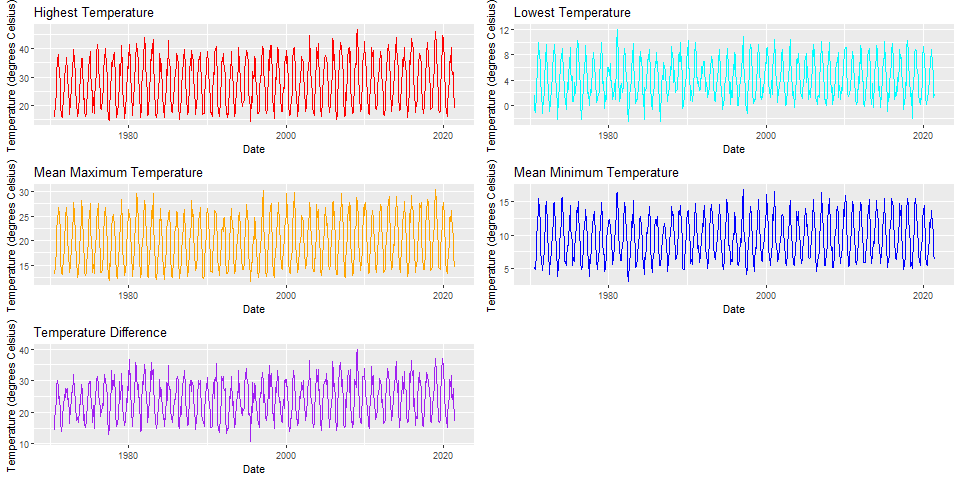
\includegraphics[scale=0.5]{Overall}\\
\newpage
Figure 2: Monthly temperature features over time\\
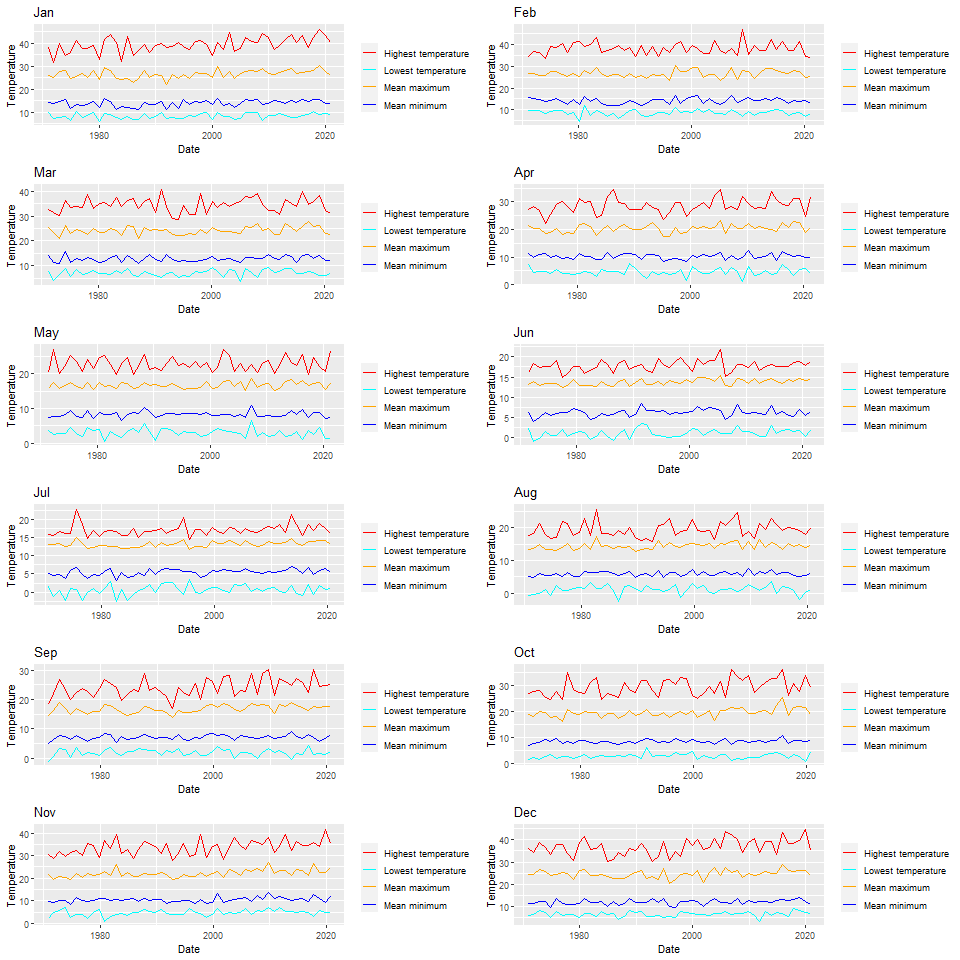
\includegraphics[scale=0.5]{Monthly}\\
Figure 3: Global warming STL decomposition\\
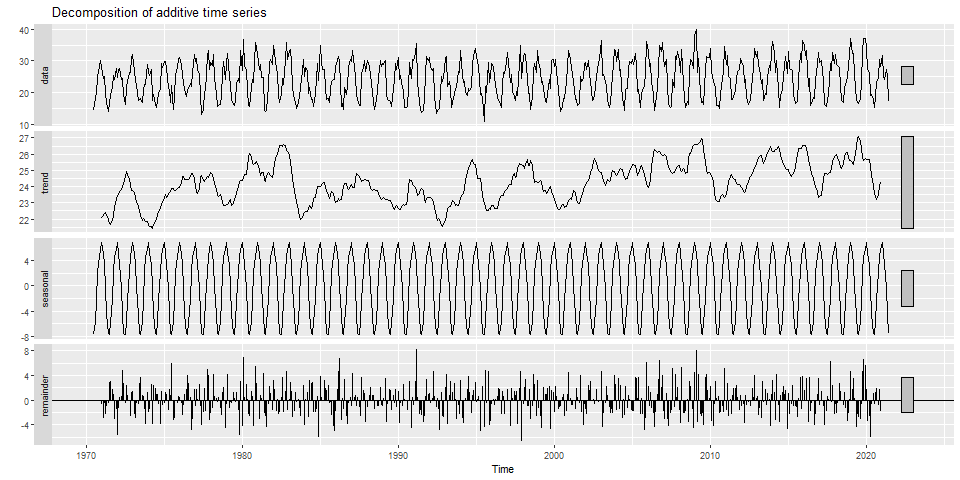
\includegraphics[scale=0.5]{GW STL}\\
Figure 4: Climate change STL decomposition\\
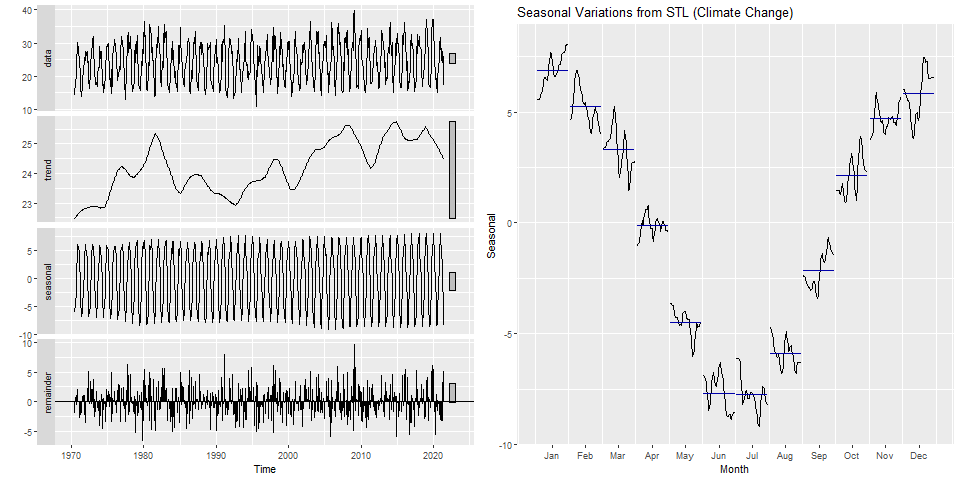
\includegraphics[scale=0.5]{CC STL}\\

\begin{table}[H] \centering 
\parbox{.45\linewidth}{
  \caption{Global Warming Regression} 
  \label{} 
\begin{tabular}{@{\extracolsep{5pt}}lcc} 
\\[-1.8ex]\hline 
\hline \\[-1.8ex] 
 & \multicolumn{2}{c}{\textit{Maximum.temperature}} \\ 
\cline{2-3} 
\\[-1.8ex] & Linear & Quadratic \\ 
\hline \\[-1.8ex] 
(Intercept) & 25.82 & 26.190 \\ 
  & (0.208) & (0.0.239) \\ 
trend & 0.002 & -0.001 \\ 
  & (0.0003) & (0.001) \\ 
trend$^2$ &  & 0.000006 \\ 
  &  & (0.000002) \\ 
season2 & 0.027 & 0.0270 \\ 
  & (0.263) & (0.261) \\ 
season3 & -2.362 & -2.362 \\ 
  & (0.263) & (0.261) \\ 
season4 & -6.190 & -6.190 \\ 
  & (0.263) & (0.261) \\ 
season5 & -9.884 & -9.884 \\ 
  & (0.263) & (0.261) \\ 
season6 & -12.860 & -12.860 \\ 
  & (0.263) & (0.261) \\ 
season7 & -13.380 & -13.380 \\ 
  & (0.263) & (0.261) \\ 
season8 & -12.120 & -12.120 \\ 
  & (0.263) & (0.261) \\ 
season9 & -9.800 & -9.800 \\ 
  & (0.263) & (0.261) \\ 
season10 & -7.038 & -7.038 \\ 
  & (0.263) & (0.261) \\ 
season11 & -4.413 & -4.413 \\ 
  & (0.263) & (0.261) \\ 
season12 & -1.900 & -1.900 \\ 
  & (0.263) & (0.261) \\ 
\hline \\[-1.8ex] 
Observations & 612 & 612 \\ 
Adjusted R$^{2}$ & 0.9278 & 0.9288 \\ 
\hline 
\hline
\end{tabular} 
}
\hfill
\parbox{.45\linewidth}{
  \caption{Climate Change Regression} 
  \label{} 
\begin{tabular}{@{\extracolsep{5pt}}lcc} 
\\[-1.8ex]\hline 
\hline \\[-1.8ex] 
 & \multicolumn{2}{c}{\textit{Difference}} \\ 
\cline{2-3} 
\\[-1.8ex] & Linear & Quadratic \\ 
\hline \\[-1.8ex] 
(Intercept) & 30.040 & 30.260 \\ 
  & (0.437) & (0.505) \\ 
trend & 0.0035 & 0.001 \\ 
  & (0.0006) & (0.003) \\ 
trend$^2$ &  & 0.00000035 \\ 
  &  & (0.000004) \\ 
season2 & -1.768 & -1.768 \\ 
  & (0.552) & (0.552) \\ 
season3 & -3.591 & -3.591 \\ 
  & (0.552) & (0.552) \\ 
season4 & -7.073 & -7.073 \\ 
  & (0.552) & (0.552) \\ 
season5 & -11.350 & -11.350 \\ 
  & (0.552) & (0.552) \\ 
season6 & -14.480 & 14.480 \\ 
  & (0.552) & (0.552) \\ 
season7 & -14.630 & 14.630 \\ 
  & (0.552) & (0.552) \\ 
season8 & -12.720 & -12.720 \\ 
  & (0.552) & (0.552) \\ 
season9 & -9.002 & -9.002 \\ 
  & (0.552) & (0.552) \\ 
season10 & -4.762 & -4.762 \\ 
  & (0.552) & (0.552) \\ 
season11 & -2.148 & -2.148 \\ 
  & (0.552) & (0.552) \\ 
season12 & -1.014 & -1.014 \\ 
  & (0.552) & (0.552) \\ 
\hline \\[-1.8ex] 
Observations & 612 & 612 \\ 
Adjusted R$^{2}$ & 0.9278 & 0.9288 \\ 
\hline 
\hline
\end{tabular} 
}
\end{table} 

Figure 5:\\
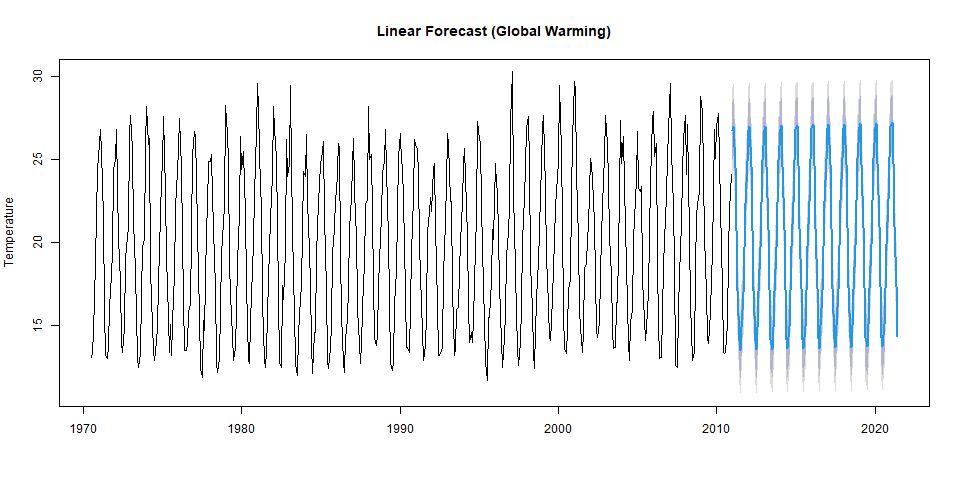
\includegraphics[scale=0.5]{Linear GW}\\
Figure 6:\\
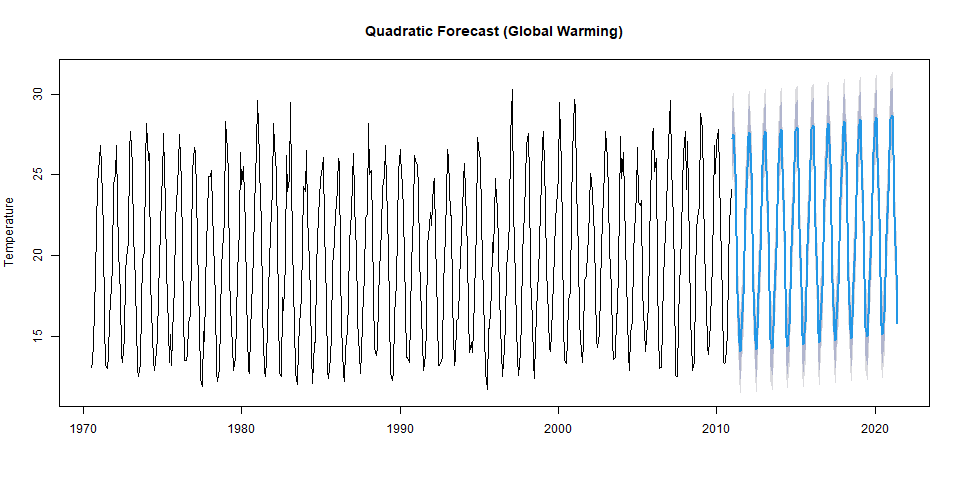
\includegraphics[scale=0.5]{Quadratic GW}\\
Figure 7:\\
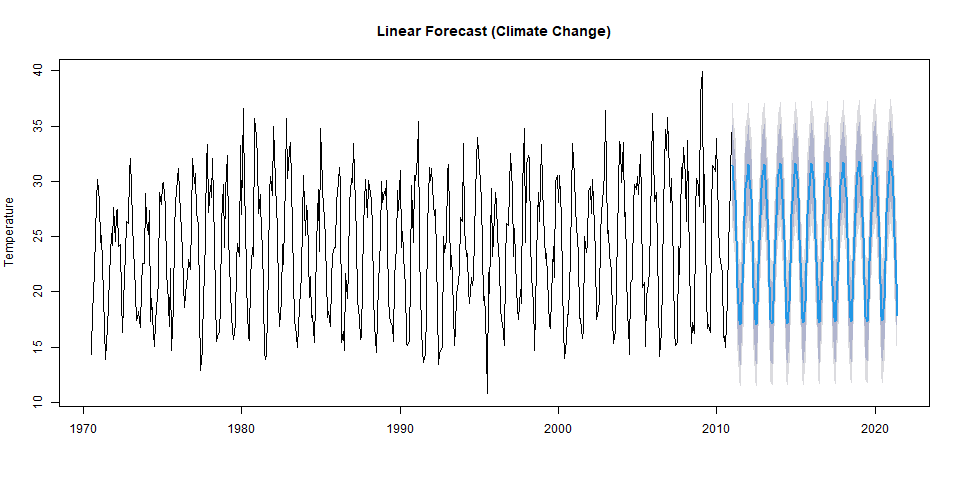
\includegraphics[scale=0.5]{Linear CC}\\
Figure 8:\\
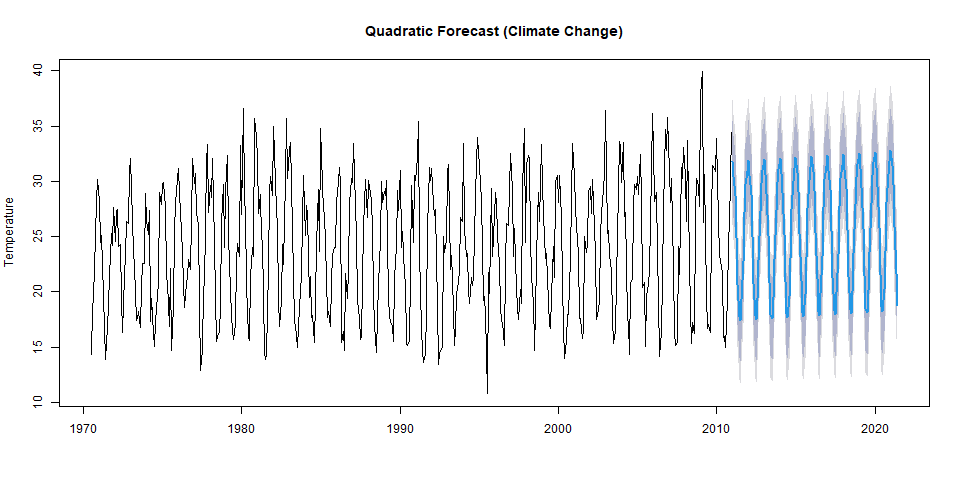
\includegraphics[scale=0.5]{Quadratic CC}\\
}
\end{document}